\documentclass[12pt]{article}
\usepackage[utf8]{inputenc}
\usepackage[a4paper, left=1in, right=1in, top=1in, bottom=1in]{geometry}
\usepackage{amsmath}
\usepackage{amssymb}
\usepackage{blindtext}
\usepackage{caption}
\usepackage{enumitem}
\usepackage{environ}
\usepackage{float}
\usepackage{graphicx}
\usepackage{indentfirst}
\usepackage{multicol}
\usepackage{setspace}
\usepackage{subcaption}
\usepackage{svg}
\usepackage{tabularx}
\usepackage{tikz}
\usepackage{titlesec}   
\usepackage{xurl}

\newcommand{\HRule}[1]{\rule{\linewidth}{#1}}
\newcommand\tab[1][1cm]{\hspace*{#1}}
\newcommand{\sref}[1]{\textsuperscript{\ref{#1}}}
\NewEnviron{slist}[1][0] {
    \setlist{nolistsep}
    \begin{itemize}[noitemsep]
        \BODY
    \end{itemize}
}

\captionsetup{justification=centering}
\DeclareMathAlphabet{\mathbfit}{OML}{cmm}{b}{it}
\graphicspath{{images/}}
\pagestyle{headings}
\setcounter{tocdepth}{5}
\setcounter{secnumdepth}{5}

\title { 
    \normalsize \textsc{}
    \\ [2.0cm]
    \HRule {3pt} \\
    \LARGE \textbf {
        MA 485V - Non-Linear Dynamic Systems \\
        Final Project \\
    }

    \HRule{3pt} \\ [0.5cm]
    
    {
        \textbf {
            Celestial \& Orbital Mechanics
        }

        {
            Modelling Celestial Motion Through Kepler's Laws \& the N-Body Problem.
        }
    }
}

\author {
    Nausher Rao\thanks{with special thanks to Dr. Ilias S. Kotsireas}
}

\date {
    \textbf{December 22\textsuperscript{nd}, 2023}
}


\begin{document}
\maketitle
\newpage
\tableofcontents


\begin{spacing}{1.25}
\newpage
\section{Abstract}
\par {
    This research report aims to comprehensively explore how we can model a non-linear dynamical system such as the motion of multiple massive celestial bodies that gravitationally interact with each other, such as the Solar System\sref{app:solar_system}. This report wants to show the different types of simulations that can be employed, the advantages and disadvantages of each, and the mathematical concepts of the n-body problem and Kepler's Laws.
}


\newpage
\section{Introduction}
\par {
    Understanding the complex non-linear mechanics that govern celestial dynamics is crucial for understanding the complexities of our planet's history and predicting the future. This research paper aims to delve into Kepler's laws of planetary motion, the n-body problem, n-body simulations, and planetary motion, and will seek to explain how they work in the present and future, and how we can model them. 
    \begin{itemize}
      \item x
    
      \item By diving into the intricacies of Kepler's laws of planetary motion, this research endeavours to show what is used in modelling the movement of the Earth in space.
      
      \item Through a comprehensive exploration of the orbital elements, this paper aims to provide a comprehensive overview of what is needed in modelling the orbital mechanics of the Earth. 
    \end{itemize}
}

\newpage
\section{\boldmath{\(n\)\text{-body Problem}}}
\subsection{Background}
\par {
    The \(n\)-body problem is the problem associated with predicting the individual motions of a group of celestial objects interacting with each other gravitationally - the system is often dynamically chaotic. More specifically, there are a variety of different approximations, analytical solutions\sref{app:analytical_solution}, numerical solutions, and complete solutions under specific closed conditions - there doesn't exist a general closed-form solution\sref{app:closed_form}. The problem increases in difficulty when relativistic effects are considered from general relativity, such as time and space distortions.

    Newton first derived simple equations for the motion of an orbiting body through straightforward analytical geometry and could calculate the position, orbital diameter, period, and orbital velocity of a planet. After a few years, he realized that the equations didn't predict certain orbits accurately. He later realized this was due to the gravitational interactions among all bodies with each other, which constantly modified the orbital paths. 
}

\subsection{Classsical Central-Force Problem}
\par {
    The \(n\)-body problem is an applied case of the \textbf{classical central-force problem}. The central-force problem is a problem from classical mechanics concerned with determining the position of a particle undergoing a central force in a central potential field - a sort of "one-body problem". A central force is defined as a force that points from the particle in question to a central fixed-point particle. Denoting the central-force particle as \(\mathbf{O}\)) and the particle as \(\mathbf{P}\), the force acting upon \(\mathbf{P}\) can be modelled as such:
    \begin{equation}
        \mathbf{F}_\mathbf{P} = F(|\mathbf{r}|) \cdot \mathbf{\hat{r}}
    \end{equation}

    \noindent where:
    \begin{slist}
        \item \(\mathbf{r}\) is a position vector that joins the \(\mathbf{O}\) to \(\mathbf{P}\).
        \item \(\mathbf{\hat{r}}\) is the unit vector of \(\mathbf{r}\).
        \item \(F\) is the central-force. \(F\) is negative when the central force is attractive, and negative if repulsive.
    \end{slist}
    
    \hfill \\
    \noindent For any object in motion, recall \textbf{Newton's second law of motion}:
    \begin{equation*}
        \mathbf{F} = m\frac{d\mathbf{v}}{dt} = m\mathbf{a}
    \end{equation*}

    \noindent where:
    \begin{slist} 
        \item \(\mathbf{F}\) is the net force being applied to the object, a vector.
        \item \(m\) is the mass of the object, a scalar.
        \item \(\mathbf{v}\) is the velocity of the object, a vector.
        \item \(\mathbf{a}\) is the net acceleration the object is undergoing, a vector.
    \end{slist}
    
    \hfill \\
    \noindent Applying Newton's second law to equation (2), we get:
    \begin{equation}
        \mathbf{F}_\mathbf{P} = F(|\mathbf{r}|) \cdot \mathbf{\hat{r}} = m\mathbf{a} = m\frac{d^2\mathbf{r}}{dt^2}
    \end{equation}

    \noindent where:
    \begin{slist}
        \item \(m\) is the mass of \(\mathbf{P}\).
        \item \(\mathbf{a}\) is the acceleration of the particle, which can be defined as the second derivative of the position vector.
    \end{slist}
}


\subsection{Two-Body Problem}
\par {
    The two-body problem is a step up from the central-force problem which considers a system with two celestial gravitational bodies. This system was completely solved by Johann Bernoulli in the case where one body was a fixed point mass. Using equation (1), the following example outlines this system using the Earth-Sun system, with all Earth-related values subscripted with \(e\) and Sun-related values with \(s\):
    \begin{subequations}
        \begin{equation}
            F_s = m_s a_s = G\frac{m_sm_e}{(r_s - r_e)^2} \: \hat{r}_{s,e}
        \end{equation}
        \begin{equation}
            F_e = m_e a_e = G\frac{m_em_s}{(r_e - r_s)^2} \: \hat{r}_{e,s}
        \end{equation}
    \end{subequations}
}

\par {
    There are a few issues with this general solution. The above equations are an idealization of a perfect situation in which two perfectly uniform and circular point masses interact with each other, without considering general relativity or other complex phenomena, such as virtual particles from quantum-field theory.
}x


\subsection{Three-Body Problem}
\par {
    The problems as mentioned earlier increase in difficulty and complexity with 3 bodies due to the chaoticness of the system. Denoting the positional vector of 3 celestial bodies with \(\bar{a}\), \(\bar{b}\), and \(\bar{c}\), the following set of nine second-order differential equations is commonly used to model said system:
    \begin{subequations}
        \begin{subequations}
            \begin{equation}
                a_x = -G \left( \frac{m_b}{(a_x - b_x)^2} + \frac{m_c}{(a_x - c_x)^2} \right)
            \end{equation}
            \begin{equation}
                a_y = -G \left( \frac{m_b}{(a_y - b_y)^2} + \frac{m_c}{(a_y - c_y)^2} \right)
            \end{equation}
            \begin{equation}
                a_z = -G \left( \frac{m_b}{(a_z - b_z)^2} + \frac{m_c}{(a_z - c_z)^2} \right)
            \end{equation}
        \end{subequations}
        
        \begin{subequations}
            \begin{equation}
                b_x = -G \left( \frac{m_a}{(b_x - a_x)^2} + \frac{m_c}{(b_x - c_x)^2} \right)
            \end{equation}
            \begin{equation}
                b_y = -G \left( \frac{m_a}{(b_y - a_y)^2} + \frac{m_c}{(b_y - c_y)^2} \right)
            \end{equation}
            \begin{equation}
                b_z = -G \left( \frac{m_a}{(b_z - a_z)^2} + \frac{m_c}{(b_z - c_z)^2} \right)
            \end{equation}
        \end{subequations}

        \begin{subequations}
            \begin{equation}
                c_x = -G \left( \frac{m_a}{(c_x - a_x)^2} + \frac{m_b}{(c_x - b_x)^2} \right)
            \end{equation}
            \begin{equation}
                c_y = -G \left( \frac{m_a}{(c_y - a_y)^2} + \frac{m_b}{(c_y - b_y)^2} \right)
            \end{equation}
            \begin{equation}
                c_z = -G \left( \frac{m_a}{(c_z - a_z)^2} + \frac{m_b}{(c_z - b_z)^2} \right)
            \end{equation}
        \end{subequations}
    \end{subequations}

    \hfill \\
    \noindent Where each of the nine equations above represents a component of the positional vectors:
    \begin{subequations}
        \begin{equation}
            \bar{a} = \langle a_x, a_y, a_z \rangle
        \end{equation}
        \begin{equation}
            \bar{b} = \langle b_x, b_y, b_z \rangle
        \end{equation}
        \begin{equation}
            \bar{c} = \langle c_x, c_y, c_z \rangle
        \end{equation}
    \end{subequations}
}


\subsection{Restricted Three-Body Problem Solution}
\par {
    As the aforementioned second-order ODEs\sref{app:ode} have no closed solutions, there exists a closed-form solution for a situation where one of the three bodies has negligible mass and is completely under the gravitational influence of the other two bodies. In this situation however, the same issues and restrictions from the two-body problem apply, but is a great way to simulate a system where one body is a dwarf planet\sref{app:dwarf_planet} or another negligibly massed body.
}


\subsection{Analytical Three-Body Problem Solution}
\par {
    Karl Fritiof Sundman\sref{app:sundman}, a Finnish mathematician, showed in 1912 that an analytical solution exists to the three-body problem. He used a power series in terms of powers of \(t^{\frac{1}{3}}\). This solution has a couple of issues of its own:
    \begin{itemize}
        \item The solution does converge for all real values of \(t\), except in the circumstance where there is zero initial angular momentum. This isn't a big issue, however, as modelling a celestial system with zero initial angular momentum is nearly never needed.
        \item Calculating values that would have enough accuracy and precision would take too many terms to be practical. In 1930, it was calculated that there would need to be \(10^{8,000,000}\) terms for an accurate representation.
    \end{itemize}
}


\subsection{Generalized \(\mathbfit{n}\)\text{-body Problem}}
\par {
    As shown by the above solutions for the three-body problem, it is quite difficult to derive solutions for such a comprehensive system of second-order ordinary differential equations. This problem is exacerbated and nearly impossible to solve for a system \(n > 3\). In four-body problem situations, the bicircular restricted four-body problem can be applied. This is where the orbit of a fourth body is negligible when compared to the other three massive bodies, and all orbits are circular orbits, with the barycenter of the system at their foci. There are quite a few methods of simulating the n-body problem by applying specific simulation algorithms:
}

\par {
    For a system with few bodies, a direct method of computation called the "particle-particle" calculation can be applied to calculate the total potential energy for each body:
    \begin{equation*}
        U_i = G \sum_{1 \leq i \leq j \leq n}^{n}{ \frac{m_im_j}{\sqrt{|| q_j - q_i ||^2}} }
    \end{equation*}

    \noindent where:
    \begin{slist}
        \item \(U_i\) is the total potential energy of the \(i\)th celestial body.
        \item \(m_i\) is the mass of the \(i\)th celestial body.
        \item \(m_j\) is the mass of the \(j\)th celestial body.
        \item \(q_i\) is the position of the \(i\)th celestial body.
        \item \(q_j\) is the position of the \(j\)th celestial body.
        \item \(G\) is the universal gravitational constant.
    \end{slist}
}

\hfill
\par {   
    The issue arises since every celestial body is treated as a particle in a chaotic system. The simplification of a complex body to a particle causes small errors in calculations. Since the system is chaotic, small errors in integration grow exponentially in time - such a simulation running over large periods will exponentially accumulate errors, making the model severely inaccurate after many iterations.
}

\par {
    A few different methods can be used to simulate an n-body system with many bodies, such as "fast multipole", "particle mesh", "PM-tree", or "mean field" methods. The issue with most of these simulations is the time complexity tending towards \(O(n^2)\), which comes with a heavy computational toll to the point of needing large-scale systems.
}




\newpage
\section{Kepler's Law of Planetary Motion}
\subsection{Background}
\par {
    Johannes Kepler, a German polymath, published his \textit{Kepler's laws of planetary motion} sometime between 1609 and 1616. Up until this point in history, Nicolaus Copernicus's \textit{Heliocentric\sref{app:heliocentric} model of the Universe} was the leading belief among the majority. This model described the Sun as a static and fixed body at the centre of the Universe, with all planets orbiting at uniform speeds and circular orbits. Copernicus used epicycles\sref{app:epicycles} to describe the variations in the apparent retrograde motion of various observable celestial bodies.
}

\par {
    Later, Sir Isaac Newton\sref{app:newton} proved that Kepler’s laws perfectly describe planetary motion, given the following parameters:
    \begin{itemize}
        \item The gravitational force was defined using an inverse r-squared law:
        \begin{equation}
            \mathbfit{\hat{F}} = G\frac{m_1m_2}{r^2} \mathbfit{\hat{r}}
        \end{equation}

        where:
        \begin{slist}
            \item \(\hat{F}\) is the force acting upon the body.
            \item \(m_1\) is the mass of the object in question.
            \item \(m_2\) is the mass of the other object.
            \item \(r\) is the distance between both bodies, \(\mathbfit{\hat{r}}\) being the unit vector for this quantity.
            \item \(G\) is the universal gravitational constant.
        \end{slist}
        
        \item The planet in question's mass was negligible with respect to the Sun's mass, given that the only gravitational force on the planet was the Sun's.
        
        \item The planet hasn't achieved escape velocity.
    \end{itemize}
    \noindent Due to these properties, Kepler's laws aren't true laws as such but are approximate observations that are quite close to reality. Perfectly modelling the movement of gravitationally massive bodies requires solving the \(\mathbfit{n}\)\textbf{-body problem}.
}







\subsection{Kepler's First Law}
\par {
    Kepler's first law states the orbit of every planet is an ellipse with the Sun at one of the two foci. The standard equation of an ellipse is as follows: 
    \begin{equation*}
        \frac{x^2}{a^2} + \frac{y^2}{b^2} = 1
    \end{equation*}
    \begin{slist}
        \item \(\mathbf{a}\) is the radius of the semi-major axis.
        \item \(\mathbf{b}\) is the radius of the semi-minor axis.
        \item \(\mathbf{x}\) and \(\mathbf{y}\) are the parameters of the multi-variable equation.
    \end{slist}

    \hfill \\
    \noindent We can use a modified version of this formula that defines an ellipse in terms of one of its focus points (where \(\epsilon\) is the eccentricity of the ellipse):
    \begin{equation}
        \left( \frac{x + a\epsilon}{a} \right)^2 + \left( \frac{y}{b} \right)^2 = 1
    \end{equation}

    \noindent From this, we can derive the polar form\sref{app:polar_form} of an ellipse by substituting \(x = r \, cos(\theta) \), \(y = r \, sin(\theta)\), \(b = a \, \sqrt{1 - \epsilon^2}\). For convenience, we are also going to create arbitrary variables to simplify the computation by letting \(k = (1 - \epsilon^2\)), and \(\mu = 2a\epsilon cos(\theta)\).
    \begin{equation*}
        a=b
    \end{equation*}

    \noindent After substitution, the formula above becomes: 
    \begin{equation*}
        \begin{split}
            r^2 \frac{1 - \epsilon^2\cos^2(\theta)}{1-e^2} &+ r(2a\epsilon\cos(\theta)) - (a^2(1 - \epsilon^2)) = 0 \\
            r^2 \frac{1 - \epsilon^2\cos^2(\theta)}{k} &+ r\mu - ka^2 = 0
        \end{split}
    \end{equation*}
    
    \noindent After this, we can apply the quadratic formula to solve for \(r\):
    \begin{equation*}
        \begin{split}    
            r_{1, 2} &= \frac{
                -\mu \pm \sqrt{ \mu^2 + 4(\frac{1 - \epsilon^2\cos^2{\theta}}{k})(a^2k) }
            }{
                2( \frac{1 - \epsilon^2\cos^2{\theta}}{k} )
            } \\
            r_{1, 2} &= \frac{-\mu \pm \sqrt{4a^2}}
            {
                2( \frac{1 - \epsilon^2\cos^2{\theta}}{k} )
            } \\
            r_{1, 2} &= k \frac{-a(\epsilon\cos{\theta} \pm 1)}
            {
                (1 + \epsilon\cos{\theta})(1 - \epsilon\cos{\theta})
            }
        \end{split}
    \end{equation*}

    \hfill \\
    \noindent And we end up with the solutions:
    \begin{equation*}
        r_1 = \frac{-a(1 - \epsilon^2)}{(1 - \epsilon\cos{\theta})}
        \text{ and }
        r_2 = \frac{a(1 - \epsilon^2)}{(1 + \epsilon\cos{\theta})}
    \end{equation*}

    \hfill \\
    \noindent If we clean up some of the terms and use \(r_2\), we end up with:
    \begin{equation}
        r(\theta) = \frac{p}{1 + \epsilon\cos{\theta}}
    \end{equation}

    \noindent where: 
    \begin{slist}
        \item \(\epsilon\) is the eccentricity of the ellipse, \(0 < \epsilon < 1\).
        \item \(r\) is the linear distance between the orbiting body and the central body in terms of the current angle of the orbiting body around its orbit.
    \end{slist}
}

\hfill \\
\par {
    \noindent Some observations can be made about certain positions of an orbiting body around its central body:
    \begin{itemize}
    \begin{subequations}
        \item The point where the orbiting body is closest to the central body is known as \textbf{perihelion}:
            \begin{equation}
                r_{min} = \frac{p}{1 + \epsilon}
            \end{equation}
        This is also the point at which the velocity of the orbiting body will be greatest.
        
        \item The point where the orbiting body is furthest from the central body is known as \textbf{aphelion}:
        \begin{equation}
            r_{max} = \frac{p}{1 - \epsilon}
        \end{equation}
        This is also the point at which the velocity of the orbiting body will be slowest.
    \end{subequations}
    \end{itemize}
}

\par {
    \noindent This ellipse formula can further be used to calculate the radius of the semi-major and semi-minor axis:
    \begin{itemize}
    \begin{subequations}
        \item The semi-major axis can be defined as the \textbf{arithmetic mean} of the aphelion and perihelion distances:
        \begin{equation}
            a = \frac{r_{max} + r_{min}}{2} = \frac{p}{1 - \epsilon^2}
        \end{equation}
    
        \item The semi-minor axis can be defined as the \textbf{geometric mean} of the aforementioned values:
        \begin{equation}
            b = \sqrt{r_{max} \, r_{min}} = \frac{p}{\sqrt{1 - \epsilon^2}}
        \end{equation}
    \end{subequations}
    \end{itemize}
}


\subsection{Kepler's Second Law}
\par {
    \textbf{Kepler's second law} states that a line joining a planet and the Sun sweeps out equal areas during intervals of time. To elaborate, if a planet travels around its orbital path for a certain amount of time \(t\), it will have travelled a distance we can call \(d_1\). Now, if anywhere else on the orbital path the planet travels the same amount of time, it will have travelled a distance of \(d_2\). Kepler's second law states that if you connect a line from the Sun to the start and endpoints of both \(d_1\) and \(d_2\), the area of both shapes is equal, therefore implying that the conservation of angular momentum holds. 
}

\begin{figure}[H]
    \centering
    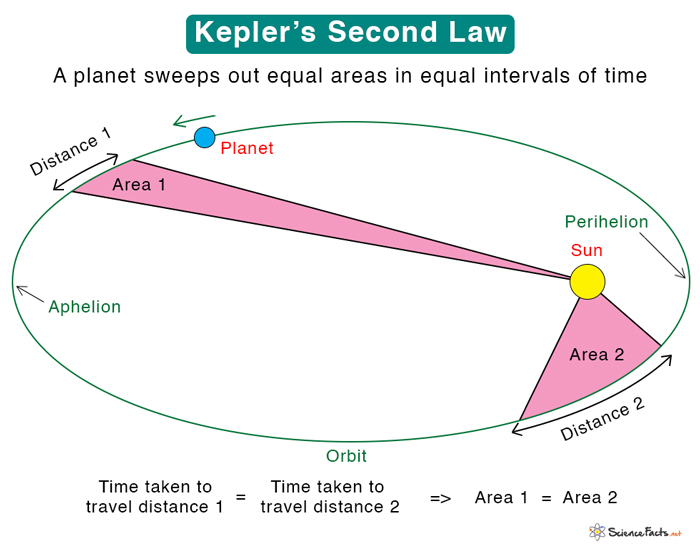
\includegraphics[height=3.5in]{images/second_law.png}
    \caption{A diagram showcasing the properties in association with Kepler's second law. Both equal areal velocities are denoted in pink.}
\end{figure}

\subsubsection{Conservation of Angular Momentum}
\par {
    Regular momentum (linear momentum) is the dot product of the mass and velocity of an object, denoted by \(\mathbf{p}\) and calculated using:
    \begin{equation*}
        \mathbf{p} = m\mathbf{v}
    \end{equation*}
    
    \noindent where:
    \begin{slist}
        \item \(m\) is the object's mass, a scalar.
        \item \(\mathbf{v}\) is the object's velocity, a vector.
    \end{slist}
    
    \hfill \\
    Angular momentum is a pseudovector\sref{app:pseudovector} that represents momentum in a rotational or orbital setting rather than a linear setting, denoted by \(L\). A fundamental law of angular momentum is known as the \textbf{Conservation of Angular Momentum}, which states that the total angular momentum of a closed system remains constant. The orbital angular momentum of a body in a circular orbit is defined as:
    \begin{equation}
        L = 2\pi Mfr^2
    \end{equation}

    \noindent where:
    \begin{slist}
        \item \(M\) is the mass of the orbiting body.
        \item \(f\) is the orbital frequency of the body.
        \item \(r\) is the radius of the orbit.
    \end{slist}
}
\hfill 
\par {
    The previously mentioned classical central-force problem lends itself well to Kepler's second law. One of the properties of the central-force problem is \textbf{constant areal velocity}. Areal velocity is defined as a pseudovector whose area is equal to the magnitude of the area that is swept out
    
    The ratio between the magnitude of the angular momentum and the mass of the particle (known as the \textbf{specific angular momentum}) equals twice the areal velocity. Since angular momentum is conserved, the areal velocity stays constant.
}


\subsubsection{Derivation}
\par {
    The derivation for Kepler's second law can be found through the equation of a triangle:
    \begin{figure}[H]
        \centering
        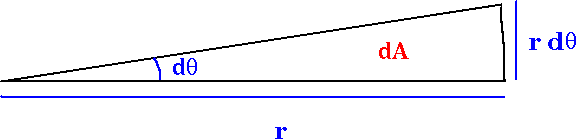
\includegraphics[width=5in]{images/kepler_triangle.png}
        \caption{A small wedge on an ellipse, represented by a triangle.}
        \label{fig:triangle}
    \end{figure}

    \noindent where:
    \begin{slist}
        \item \(dA\) is the area of this infinitesimal triangle.
        \item \(r\) is the base of the triangle - the distance from the centre to the circumference.
        \item \(rd\theta\) is the height of the triangle. Since the triangle is infinitesimal, we can consider the height to be vertically straight rather than curved.
    \end{slist}

    \noindent We can then use this to calculate the area:
    \begin{equation*}
        dA = \frac{1}{2}(r)(rd\theta)
    \end{equation*}

    \noindent We can then divide by the time differential (\(dt\)) to get the rate at which the area is swept out at:
    \begin{equation}
        \begin{split}
            \frac{dA}{dt} = \frac{1}{2}(r)(r\frac{d\theta}{dt}) = \frac{1}{2}r\nu_\theta
        \end{split}
    \end{equation}

    \begin{subequations}
        \noindent We can then use the equation for angular momentum for a simplified circular system:
        \begin{equation}
            \begin{split}
                \mathbf{L} & = m(\mathbf{r} \times \mathbf{\nu}) \\
                L & = mr\nu_\theta
            \end{split}
        \end{equation}
    
        \noindent Re-arranging equation (11a):
        \begin{equation}
            \frac{L}{m} = r\nu_\theta
        \end{equation}
    \end{subequations}

    \hfill \\
    \noindent We can then substitute equation (11b) into equation (10):
    \begin{equation}
        \frac{dA}{dt} = \frac{1}{2}\frac{L}{m}
    \end{equation}

    \noindent This implies that for a central line joining two points over a given period of time around the orbit, the rate at which the area that's swept out is constant.
}


\subsection{Kepler's Third Law}
\par {
    \textbf{Kepler's third law} states that the square of an object's orbital period is proportional to the cube of its semi-major axis. The purpose of this law is to show the relationship between distances at which planets orbit the Sun. This relationship can be determined through the following derivation:

    \noindent First, using the previously discussed Newton's law of universal gravitational, we set the centripetal and gravitational forces on a celestial body equal to each other:
    \begin{equation}
        ma\omega^2 = G \frac{mM}{r^2}
    \end{equation}

    \noindent where:
    \begin{slist}
        \item \(m\) is the mass of the orbiting body.
        \item \(a\) is the semi-major axis of the orbiting body.
        \item \(\omega\) is the angular velocity of the orbiting body.
        \item \(G\) is the universal gravitational constant.
        \item \(M\) is the mass of the other body that this body is attracted to.
        \item \(r\) is the distance between both bodies.
    \end{slist}

    \hfill \\
    \noindent We can then recall the definition of angular velocity expressed in terms of the orbital period (denoted by \(T\)):
    \begin{equation*}
        \omega = \frac{2\pi}{T}
    \end{equation*}

    \hfill \\
    \noindent And we can substitute this into equation (14):
    \begin{equation*}
        \begin{split}
            ma \left( \frac{2\pi}{T} \right)^2 = G \frac{mM}{r^2} \\
            T^2 = \left( \frac{4\pi^2}{GM} \right) r^3
        \end{split}
    \end{equation*}
    
    \hfill \\
    \noindent Trivially, \( \frac{4\pi^2}{G} \) is a constant term and \(M\) only depends on the other gravitational body. Therefore, we are left with the following relationship:
    \begin{equation}
        T^2 \propto r^3
    \end{equation}
}


\newpage
\section{n-body Simulation}
\subsection{Introduction}
\par {
    x
}


\subsection{Many-Body Simulations}
\par {
    x
}


\subsection{Few-Body Simulations}
\par {
    x
}


\subsubsection{Particle–Particle Method}
\par {
    x
}


\newpage
\section{Conclusion}
\par {
    The exploration into Kepler's laws and the intricacies of celestial motion and dynamics has given us a good basic understanding as to understanding how one may go about modelling the motion of gravitationally-major celestial bodies, and the benefits and drawbacks of each of the different types of simulation methods. We can also observe how that motion can be precisely calculated and modelled mathematically. Kepler's laws of planetary motion provided a celestial roadmap, dictating the gravitational laws that govern our solar system. The mathematics behind these laws has shown the precision with which celestial bodies interact through space.
}


\newpage
\section{References}
\par {
    \begin{itemize}
        \item Encyclopædia Britannica, inc. (2023a, November 5). Newton’s laws of Motion. 
        Encyclopædia Britannica. \url{https://www.britannica.com/science/Newtons-laws-of-motion} 
        
        \item Encyclopædia Britannica, inc. (2023b, November 7). Newton’s law of gravitation. 
        Encyclopædia Britannica. \url{https://www.britannica.com/science/Newtons-law-of-gravitation}
        
        \item Encyclopædia Britannica, inc. (2023c, December 8). Kepler’s laws of planetary motion. 
        Encyclopædia Britannica. \url{https://www.britannica.com/science/Keplers-laws-of-planetary-motion} 
        
        \item Encyclopædia Britannica, inc. (n.d.). Kepler’s Second Law of Planetary Motion. 
        Encyclopædia Britannica. \url{https://www.britannica.com/science/Keplers-second-law-of-planetary-motion} 
        
        \item NASA. (n.d.). Orbits and Kepler’s laws - Nasa Science. 
        NASA. \url{https://science.nasa.gov/resource/orbits-and-keplers-laws/}
                
        \item Pollard, H. (1966). Mathematical introduction to celestial mechanics. 
        Englewood Cliffs. 
        
        \item Wikimedia Foundation. (2023a, August 6). Orbital eccentricity.
        Wikipedia. \url{https://en.wikipedia.org/wiki/Orbital\_eccentricity} 
        
        \item Wikimedia Foundation. (2023b, September 1). N-body problem.
        Wikipedia. \url{https://en.wikipedia.org/wiki/N-body\_problem}
        
        \item Wikimedia Foundation. (2023c, November 28). Elliptic orbit. 
        Wikipedia. \url{https://en.wikipedia.org/wiki/Elliptic\_orbit}
        
        \item Wikimedia Foundation. (2023d, December 13). Angular momentum. 
        Wikipedia. \url{https://en.wikipedia.org/wiki/Angular\_momentum}
        
        \item Wikimedia Foundation. (2023e, December 16). Kepler’s laws of planetary motion. 
        Wikipedia. \url{https://en.wikipedia.org/wiki/Kepler\%27s\_laws\_of\_planetary\_motion}
    \end{itemize}
}
 

\newpage
\section{Appendixes}
\par {
    \begin{enumerate}                
        \item \label{app:celestial} \textbf{Celestial:} About something related to space or the sky. In general, a "celestial body" is an astronomical physical object that exists within the observable universe. 

        \item \label{app:heliocentric} \textbf{Heliocentric:} A school of thought used in old Ptolemaic and Copernican theories for astronomy that hypothesized that the Earth and planets revolve around the Sun, which is set at the center of the universe.

        \item \label{app:epicycles}\textbf{Epicycles:} Heavily involved in old Ptolemaic and Copernican theories for astronomy - epicycles were an idea used to solve the problem of the variations in speed and direction of the apparent motion of the Moon, Sun, and planets. In particular, it explained the apparent retrograde motion\sref{app:appaarent_retrograde_motion} of the five planets known at the time. Secondarily, it also explained changes in the apparent distances of the planets from the Earth.

        \item \label{app:newton} \textbf{Isaac Newton:} Sir Isaac Newton was an English polymath (mainly involved in mathematics, physics, astronomy, alchemy, and theology) who is most known for establishing classical mechanics and making major contributions to optics and developing infinitesimal calculus.

        \item \label{app:analytical_solution} \textbf{Analytical Solution}: A solution to a mathematical problem restricted by the same rule as a closed-form solution, but with additional functions that are allowed. These functions are non-algebraic polynomial roots, gamma functions, Bessel functions, and special functions.

        \item \label{app:closed_form} \textbf{Closed-Form Solution:} A solution to a mathematical problem that only contains a finite set of constants, variables, and basic functions, and only uses basic arithmetic operations and function composition. The basic functions are nth root, exponentiation, logarithmic, and trigonometric.
        
        \item \label{app:ode} \textbf{ODE:} Shorthand abbreviation for "second-order differential equation".

        \item \label{app:dwarf_planet} \textbf{Dwarf Planet:} A small planet-esque body contained within a star system.

        \item \label{app:sundman} \textbf{Karl Fritiof Sundman:} A Finnish mathematician who showed the existence of an analytical convergent infinite series solution to the three-body problem.

        \item \label{app:polar_form} \textbf{Polar Form:} A set of coordinates that use the polar coordinate system - each point on a plane is represented by a two-dimensional vector - the first value being the distance from a reference point, this usually being the origin. The second value is the angle between the ray from the point to the reference point and the origin.

        \item \label{app:pseudovector} \textbf{Pseudovector:} A quantity that behaves like a vector. A pseudovector has no guarantee of keeping Euclidean distances and direction preserved under certain transformations. 
        
        \item \label{app:keplerian_orbits} \textbf{Keplerian Orbits}: The orbital motion of one body relative to another, usually following an elliptical, parabolic, or hyperbolic path, which forms a two-dimensional orbital plane in three-dimensional space.

        \item \label{app:apparent_retrograde_motion} \textbf{Apparent Retrograde Motion:} The motion of a planet in a direction opposite to that of other bodies within its system, as observed from a particular vantage point.
    \end{enumerate}
}

\end{spacing}
\end{document}